\documentclass[./main.tex]{subfiles}

\begin{document}
\section{Finetuning}
\label{sec:finetuning}
As we now have finetuned our models, we need to finetune the models, such that they are specialized to yield optimial results on the ClimbAlong dataset. The following section describes the finetuning of these models. This includes the preprocessing of the data, the configuration details we use, as well as the obtained results.
\\
\\
In the finetuning stage we will be using the already developed pose-estiamtor to train our temporal-inclusive models. However, we will be freezing the pose-estimator, such that the weights of the model will not change during the training and we will thus only train our temporal-inclusive models. We do this for the following three reasons: (1) the training of the models will be quicker, as we just need to train the temporal-inclusive models and not the already developed pose-estimator, and (2) we get an greater understanding of the effects of our models when combined with the pose-estimator, as we can clearly see how big of a difference it makes by adding our temporal-inclusive models.

\subsection{Data Preprocessing}
For the ClimbAlong dataset we perform only minor preprocessing. First, the preprocessing of each video is done by having the already developed pose-estimator process the video, such that we have the output heatmaps of the pose-estimator, containing all of the pose-estimations of each video. Next, we preprocess the heatmaps by setting all negative values to $0$ and normalizing each heatmap, such that each heatmap sums up to the fixed value $c = 255$ that we used when preprocessing the BRACE and Penn Action datasets, essentially making the heatmaps more similar to the preprocessed heatmaps of BRACE and Penn Action. These heatmaps will then be used as the input for our models.
\\
\\
For the groundtruth heatmaps we create twenty five heatmaps of each frame, similarly to how we did it for the BRACE and Penn Action datasets, however, in this case we use the predicted bounding-box of the pose-estimator as our bounding-box. In cases where the groundtruth keypoint is placed outside of the bounding-box, we place the groundtruth keypoint at the closest border of the bounding-box.

\subsection{Training Details}
\textbf{Data Configuration} Generally, we follow a similar approach to how we did in the pretraining stage. We again use a window-size of $k = 5$ frames, resulting in a total of $9,419$ windows. Also here are we using $c = 255$ as a representation of the ground turht placement of each keypoint. We also split the dataset into a non-overlapping and non-repeating training, validation and test set, consisting of $60\%$, $20\%$ and $20\%$ of the data, respectively. However, we note that one incorrect frame can have a huge impact on the evaluation results, as this frame is used five times during evaluation, and with the small dataset these five samples can have a huge impact. For that reason, for the validation and test set we make sure that no of the windows of the same set are overlapping.
\\
\\
\textbf{Experiments} As the finetuning dataset is so small, the fitting of the models is very quick, making us fit all of the 26 developed models from the pretraining stage. For each model we pick the epoch from the pretraining stage, that yielded the highest validation accuracy and use that for finetuning.
\\
\\
\textbf{Training Configuration} The optimization parameters are very similar to the ones from the pretraining stage. We again use the ADAM optimzer with a batch size of $16$ and the MSE loss-function. During training, we again keep track of the lowest reached validation loss of an epoch and use learning-rate reduction and early-stopping in a similar manner to how we did in the pretraining stage. However, unlike the pretraining stage, we here use a smaller iniitial learning rate of $10^{-4}$, as the weights only need to be fineadjusted, making us believe that greater learning rate would skew the weights too much.

\subsection{Training and Validation Results}
\label{subsec:finetune_train_val_res}
\begin{figure}[htbp]
    \centering
     \begin{subfigure}[b]{\textwidth}
         \centering
         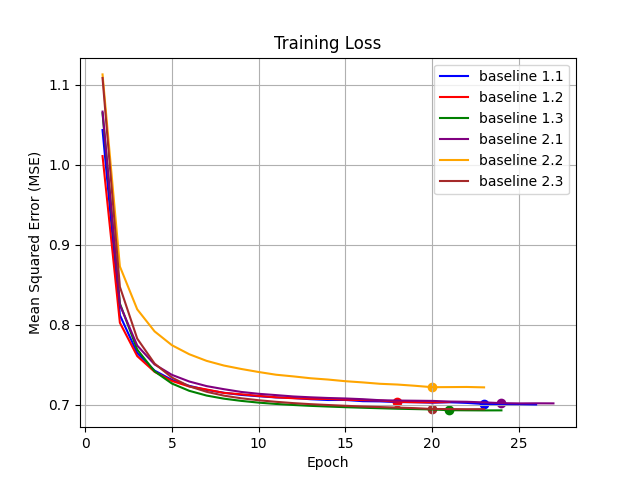
\includegraphics[width=0.32\textwidth]{./entities/finetuned/baseline/train_losses.png}
         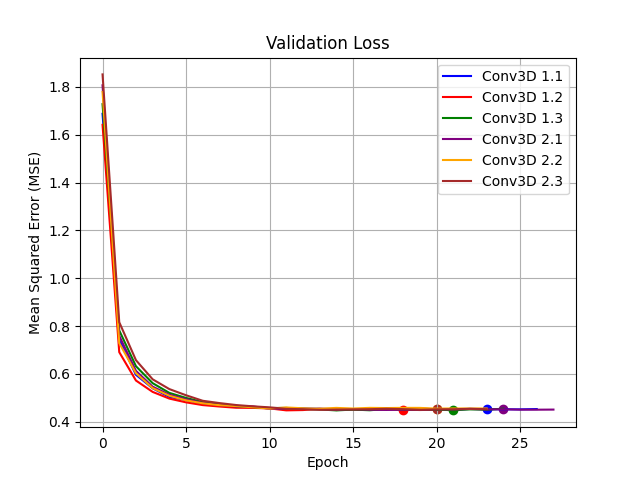
\includegraphics[width=0.32\textwidth]{./entities/finetuned/baseline/val_losses.png}
         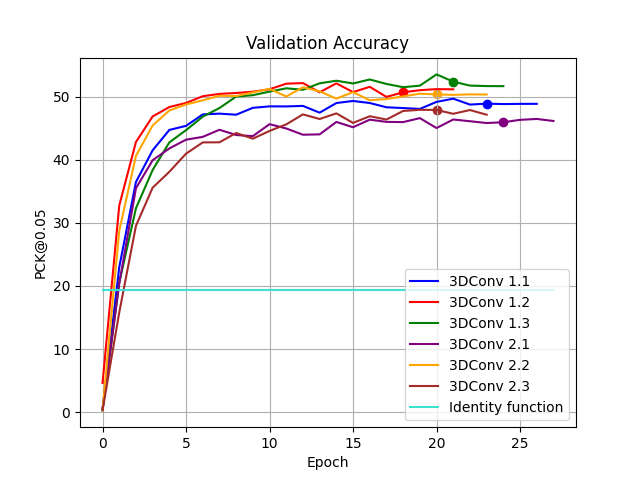
\includegraphics[width=0.32\textwidth]{./entities/finetuned/baseline/val_accs.png}
         \caption{Finetuning results of the 3-dimensional convolutional layer.}
     \end{subfigure}
    \hfill

    \begin{subfigure}[b]{\textwidth}
        \centering
        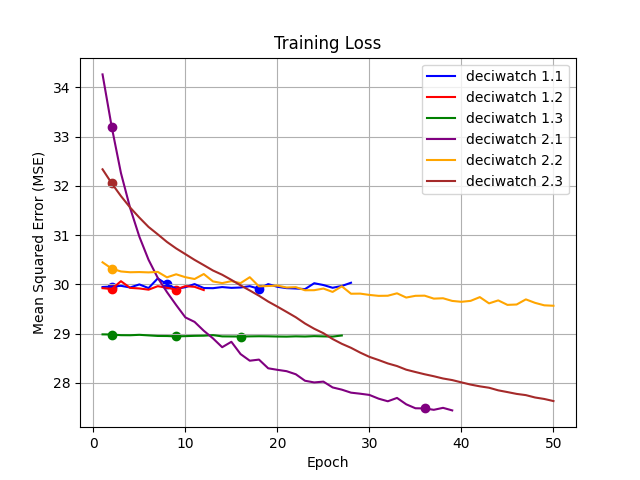
\includegraphics[width=0.32\textwidth]{./entities/finetuned/deciwatch/train_losses.png}
        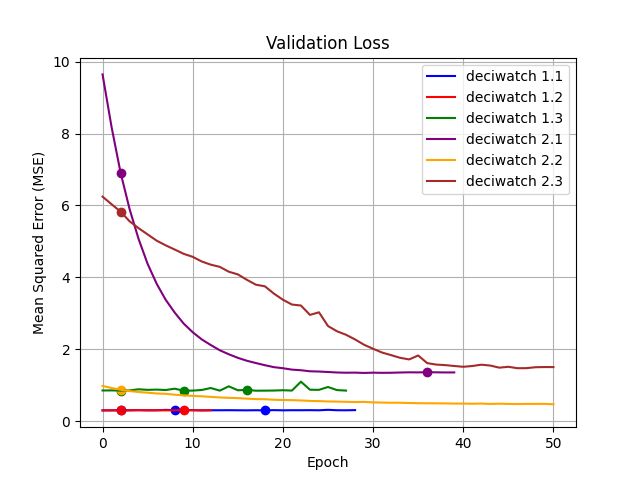
\includegraphics[width=0.32\textwidth]{./entities/finetuned/deciwatch/val_losses.png}
        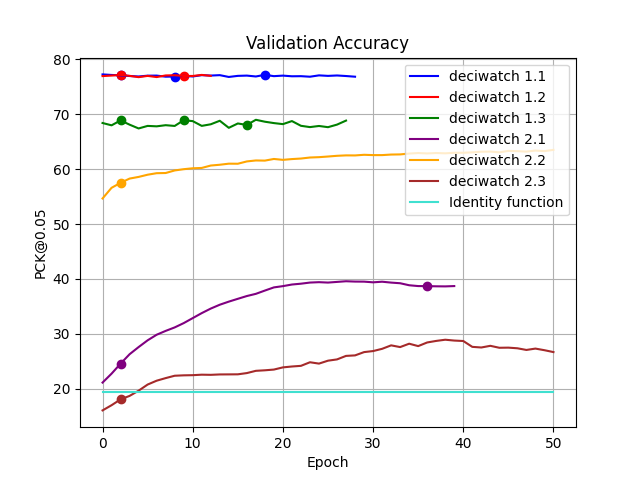
\includegraphics[width=0.32\textwidth]{./entities/finetuned/deciwatch/val_accs.png}
        \caption{Finetuning results of DeciWatch.}
    \end{subfigure}
   \hfill

   \begin{subfigure}[b]{\textwidth}
    \centering
    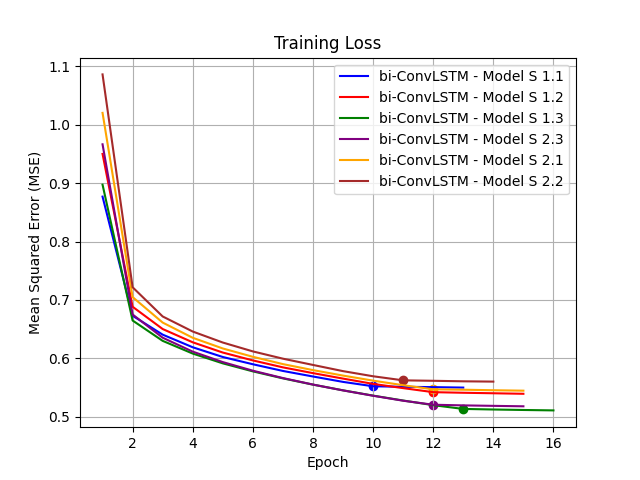
\includegraphics[width=0.32\textwidth]{./entities/finetuned/unipose/train_losses.png}
    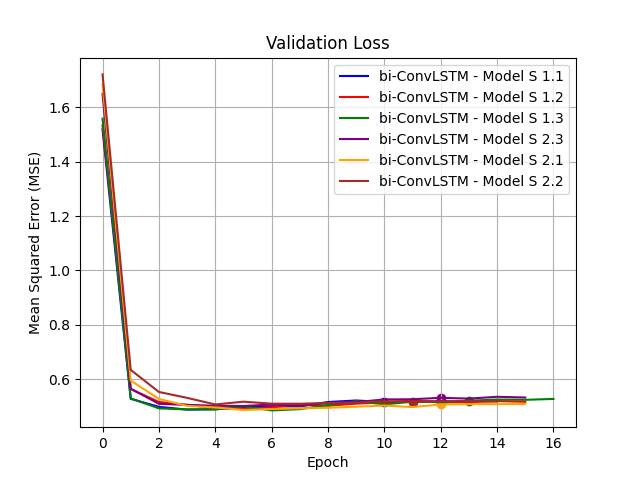
\includegraphics[width=0.32\textwidth]{./entities/finetuned/unipose/val_losses.png}
    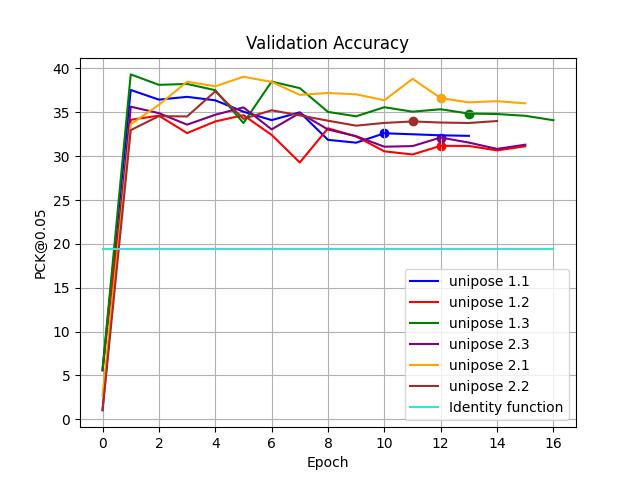
\includegraphics[width=0.32\textwidth]{./entities/finetuned/unipose/val_accs.png}
    \caption{Finetuning results of the bidirectional convolutional LSTM with summing.}
    \end{subfigure}
    \hfill

    \begin{subfigure}[b]{\textwidth}
        \centering
        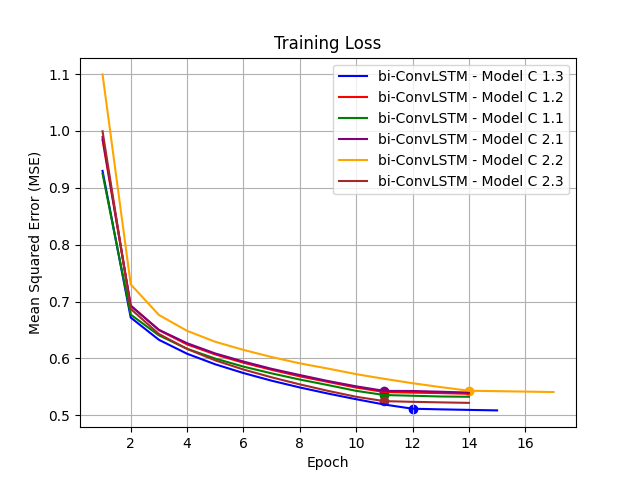
\includegraphics[width=0.32\textwidth]{./entities/finetuned/unipose2/train_losses.png}
        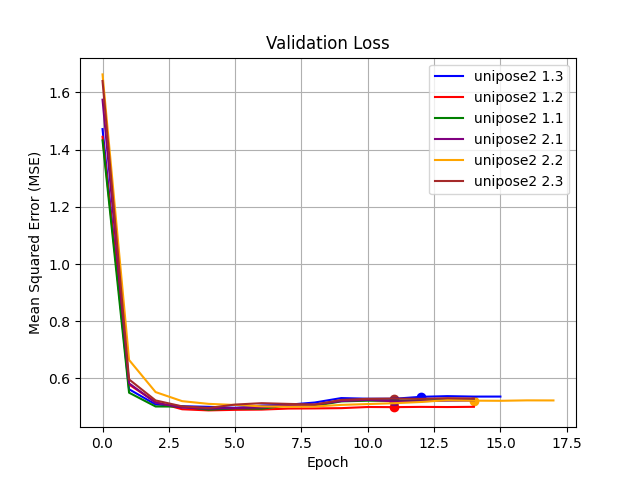
\includegraphics[width=0.32\textwidth]{./entities/finetuned/unipose2/val_losses.png}
        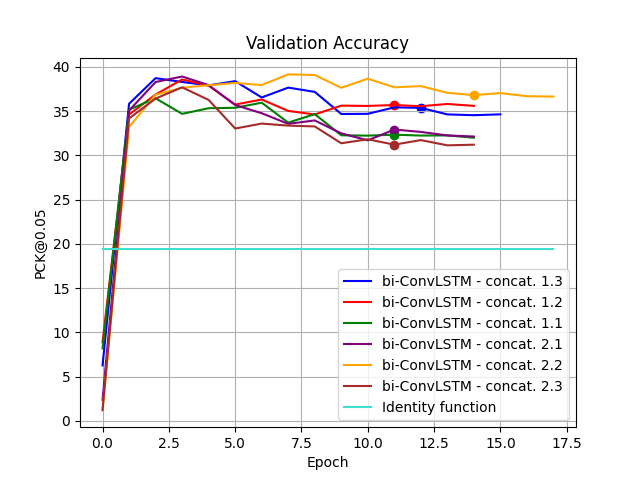
\includegraphics[width=0.32\textwidth]{./entities/finetuned/unipose2/val_accs.png}
        \caption{Finetuning results of the bidirectional convolutional LSTM with concatenation.}
    \end{subfigure}
    \hfill
    
    \caption{Evolution of the training loss, validation loss and validation PCK@0.05 accuracy of the 24 models during training, as well as the validation PCK@0.05 accuracy of the identity function of the two datasets. The dots indicates a reduction of learning-rate. First row: 3-dimensional convolutional layer. Second row: DeciWatch. Third row: Bidirectional Convolutional LSTM with summing. Fourth row: Bidirectional Convolutional LSTM with concatenation.}
    \label{fig:finetune_res}
\end{figure}

We have in Figure \ref{fig:finetune_res} illustrated the evaluation of the training loss, validation loss, and validation PCK@0.05 accuracy of the various models during the finetuning.
\\
\\
If we compare the models against the identity function we clearly see, how all models converge towards beating the identity function, indicating the positive effects of incorporating temporal information into the pose estimation of videos.
\\
\\
Further, most models tend to start off with a low validation accuracy, which could make one believe, that the pretraining has not had any effect. However, we can further see how the models tend to yield very good results after just one epoch of finetuning, making us believe that the pretraining has actually had an effect. One could argue, that a similar pattern occurred in the pretraining stage, which we would agree with. However, we have to remember that the pretraining stage contained many more samples, hence why the models were also trained on much more data in first epoch, and thus had a better likelihood of yielding good results after the first epoch, although they were not pretrained.
\\
\\
Generally, the shifting-scalar seems to only have a minor effect on the models during the finetuning, as all six runs of each model tend converge towards the same result. This however does not hold for DeciWatch, as the DeciWatch models with shifting-scalar $s = 1$ seems to be having a lot of difficulty fitting compared to all of the other models, however, they do still yield some very accurate results.

\subsection{Test Results}
\begin{table}[htbp]
    \begin{tabular}{c||ccc|ccc|ccc}
        \hline
        Accuracy metric & \multicolumn{3}{c}{PCK@0.05} & \multicolumn{3}{c}{PCK@0.1} & \multicolumn{3}{c}{PCK@0.2} \\
        \hline
        Mean threshold distance* & \multicolumn{3}{c}{0.80} & \multicolumn{3}{c}{1.60} & \multicolumn{3}{c}{3.21} \\
        \hline
        Experiment & 1.1 & 1.2 & 1.3 & 1.1 & 1.2 & 1.3 & 1.1 & 1.2 & 1.3 \\
        \hline
        \hline
        Identity function & 19.4 & 19.4 & 19.4 & 66.1 & 66.1 & 66.1 & 85.2 & 85.2 & 85.2 \\
        Conv3D & 49.7 & 52.3 & 53.1 & \textbf{95.7} & \textbf{95.7} & \textbf{95.8} & 99.2 & 99.3 & 99.3 \\
        DeciWatch & \textbf{76.9} & \textbf{76.7} & \textbf{68.7} & 94.3 & 94.4 & 86.9 & 99.2 & 99.2 & 96.2 \\
        bi-ConvLSTM - sum. & 37.8 & 34.9 & 39.0 & 91.8 & 92.1 & 92.2 & 99.4 & \textbf{99.7} & 99.2 \\
        bi-ConvLSTM - concat. & 35.9 & 39.0 & 38.5 & 93.1 & 93.6 & 92.6 & \textbf{99.8} & \textbf{99.7} & \textbf{99.7} \\
        \hline
    \end{tabular}
    \caption{Testing accuracies of the various developed models for shifting-scalar $k = 1$. All the accuracies are in percentage. *: The mean maximum distance between the predicted keypoint and corresponding groundtruth keypoint for the prediction to count as being correct, using the units of the heatmap coordinates.}
    \label{tab:finetune_test_accs_1}
\end{table}

\begin{table}[htbp]
    \begin{tabular}{c||ccc|ccc|ccc}
        \hline
        Accuracy metric & \multicolumn{3}{c}{PCK@0.05} & \multicolumn{3}{c}{PCK@0.1} & \multicolumn{3}{c}{PCK@0.2} \\
        \hline
        Mean threshold distance* & \multicolumn{3}{c}{0.80} & \multicolumn{3}{c}{1.60} & \multicolumn{3}{c}{3.21} \\
        \hline
        Experiment & 2.1 & 2.2 & 2.3 & 2.1 & 2.2 & 2.3 & 2.1 & 2.2 & 2.3 \\
        \hline
        \hline
        Identity function & 19.4 & 19.4 & 19.4 & 66.1 & 66.1 & 66.1 & 85.2 & 85.2 & 85.2 \\
        Conv3D & \textbf{46.5} & \textbf{51.6} & \textbf{47.3} & \textbf{95.5} & \textbf{95.5} & \textbf{95.8} & 99.2 & 99.3 & 99.2 \\
        DeciWatch & 34.4 & 48.9 & 32.3 & 79.4 & 69.0 & 71.6 & 95.8 & 86.3 & 92.3 \\
        bi-ConvLSTM - sum. & 38.8 & 37.4 & 35.9 & 92.7 & 92.1 & 91.2 & 99.4 & \textbf{99.5} & 99.3 \\
        bi-ConvLSTM - concat. & 39.2 & 39.5 & 37.1 & 92.5 & 92.9 & 92.6 & \textbf{99.6} & 99.3 & \textbf{99.6} \\
        \hline
    \end{tabular}
    \caption{Testing accuracies of the various developed models for shifting-scalar $k = 2$. All the accuracies are in percentage. *: The mean maximum distance between the predicted keypoint and corresponding groundtruth keypoint for the prediction to count as being correct, using the units of the heatmap coordinates.}
    \label{tab:finetune_test_accs_2}
\end{table}

\noindent We have in Table \ref{tab:finetune_test_accs_1} and Table \ref{tab:finetune_test_accs_2} illustrated the testing results of the epoch of each model that yielded the highest validation PCK@0.2 accuracy.
\\
\\
By comparing the two tables against each other we see, that the shifting-scalar tend to have a big effect on the results of DeciWatch. This is very similar to what we experienced in section \ref{subsec:finetune_train_val_res}, where we saw that the DeciWatch models with shifting-scalar $s = 1$ had a lot of difficulty fitting. For the remaining models we do see a performance difference between the two shifint-scalars, however, the performance difference is not as big as it is for DeciWatch. Generally however, the models do perform best with the noise-scalar $s = 1$.
\\
\\
Similarly to the pretraining stage, we also see here how the 3-dimensional convolutional layer from experiment 2 performs better than the 3-dimensional convolutional layer from experiment 1, however, this performance difference is now smaller than it was in the pretraining stage.
\\
\\
Further, if we look at the DeciWatch-based models we see, that the models from experiment 3 yields the worst results out of the three, similar to how it did in the pretraining stage. For the three other models, the models from experiment 3 do not seem to have any consistent major impact on the final results.
\\
\\
Like in the pretraining stage, there does not seem to be any major performance differences between the two architectures that are based on the bidirectional convolutional LSTM, making us further believe that our concern about the missing opportunity of the model to prioritize a processing direction is not that important.

\begin{table}[htbp]
    \begin{tabular}{c||ccc|ccc|ccc}
        \hline
        Accuracy metric & \multicolumn{3}{c}{PCK@0.05} & \multicolumn{3}{c}{PCK@0.1} & \multicolumn{3}{c}{PCK@0.2} \\
        \hline
        Mean threshold distance* & \multicolumn{3}{c}{0.87} & \multicolumn{3}{c}{1.77} & \multicolumn{3}{c}{3.55} \\
        \hline
        Experiment & 1.1 & 1.2 & 1.3 & 1.1 & 1.2 & 1.3 & 1.1 & 1.2 & 1.3 \\
        \hline
        \hline
        Identity function & 21.2 & 21.2 & 21.2 & 65.5 & 65.5 & 65.5 & 84.7 & 84.7 & 84.7 \\
        Conv3D & 58.4 & \textbf{61.4} & \textbf{61.7} & \textbf{98.7} & \textbf{98.9} & \textbf{99.0} & \textbf{99.6} & \textbf{99.8} & \textbf{99.7} \\
        DeciWatch & \textbf{65.1} & 56.0 & 59.6 & 93.5 & 91.1 & 89.5 & 99.1 & 98.9 & 97.6 \\
        bi-ConvLSTM - sum. & 45.7 & 45.0 & 47.6 & 97.3 & 96.9 & 97.0 & \textbf{99.6} & \textbf{99.6} & 99.1 \\
        bi-ConvLSTM - concat. & 44.5 & 46.1 & 48.5 & 97.4 & 97.9 & 97.9 & 99.6 & 99.5 & 99.6 \\
        \hline
    \end{tabular}
    \caption{Testing accuracies of the various developed models for shifting-scalar $k = 1$ on the additional test video. All the accuracies are in percentage. *: The mean maximum distance between the predicted keypoint and corresponding groundtruth keypoint for the prediction to count as being correct, using the units of the heatmap coordinates.}
    \label{tab:finetune_test_accs_3}
\end{table}

\begin{table}[htbp]
    \begin{tabular}{c||ccc|ccc|ccc}
        \hline
        Accuracy metric & \multicolumn{3}{c}{PCK@0.05} & \multicolumn{3}{c}{PCK@0.1} & \multicolumn{3}{c}{PCK@0.2} \\
        \hline
        Mean threshold distance* & \multicolumn{3}{c}{0.87} & \multicolumn{3}{c}{1.77} & \multicolumn{3}{c}{3.55} \\
        \hline
        Experiment & 2.1 & 2.2 & 2.3 & 2.1 & 2.2 & 2.3 & 2.1 & 2.2 & 2.3 \\
        \hline
        \hline
        Identity function & 21.2 & 21.2 & 21.2 & 65.5 & 65.5 & 65.5 & 84.7 & 84.7 & 84.7 \\
        Conv3D & \textbf{56.2} & \textbf{60.0} & \textbf{56.6} & \textbf{98.9} & \textbf{98.8} & \textbf{98.8} & \textbf{99.7} & \textbf{99.7} & \textbf{99.7} \\
        DeciWatch & 35.2 & 48.8 & 40.5 & 75.9 & 89.3 & 79.3 & 94.1 & 98.9 & 95.5 \\
        bi-ConvLSTM - sum. & 44.8 & 46.2 & 45.0 & 96.9 & 95.9 & 97.1 & 99.5 & 99.6 & 99.5 \\
        bi-ConvLSTM - concat. & 45.9 & 47.9 & 46.7 & 96.7 & 97.1 & 98.1 & 99.6 & 99.4 & 99.6 \\
        \hline
    \end{tabular}
    \caption{Testing accuracies of the various developed models for shifting-scalar $k = 2$ on the additional test video. All the accuracies are in percentage. *: The mean maximum distance between the predicted keypoint and corresponding groundtruth keypoint for the prediction to count as being correct, using the units of the heatmap coordinates.}
    \label{tab:finetune_test_accs_4}
\end{table}

\noindent One might argue, that our way of splitting the evaluation set into a validation and test set carries some bias, as they are so similar and that we use the validation set to pick the models that we use for testing. To test whether this is true, we have in Table \ref{tab:finetune_test_accs_3} and Table \ref{tab:finetune_test_accs_4} tested the same models on a video that have not been included in any of the other three sets. By looking at these two tables we clearly see, that none of the models perform worse than how they did in Table \ref{tab:finetune_test_accs_1} and \ref{tab:finetune_test_accs_2}, indicating that no bias was introduced when we split the evaluation data into a validation and test set.

\begin{table}[htbp]
    \begin{adjustbox}{center}
        \begin{tabular}{c||ccc|ccc|ccc|ccc|c}
            \hline
            & \multicolumn{3}{c}{Conv3D} & \multicolumn{3}{c}{DeciWatch} & \multicolumn{3}{c}{\begin{tabular}[c]{@{}c@{}}bi-ConvLSTM\\ sum.\end{tabular}} & \multicolumn{3}{c}{\begin{tabular}[c]{@{}c@{}}bi-ConvLSTM\\ concat.\end{tabular}} & Total \\ 
            \hline
            Experiment & 1.1 & 1.2 & 1.3 & 1.1 & 1.2 & 1.3 & 1.1 & 1.2 & 1.3 & 1.1 & 1.2 & 1.3 & \\
            \hline
            \hline
            Nose & 100 & 100 & 100 & 99.8 & 99.8 & 97.5 & 100 & 100 & 99.9 & 100 & 99.7 & 99.9 & \\
            Ear & 100 & 100 & 100 & 99.8 & 99.8 & 99.8 & 97.7 & 99.9 & 100 & 100 & 100 & 99.9 & \\
            Shoulder & 99.9 & 100 & 99.9 & 99.8 & 99.8 & 97.4 & 100 & 100 & 99.9 & 100 & 100 & 100 & \\
            Elbow & 99.9 & 99.9 & 99.9 & 99.4 & 99.4 & 96.9 & 100 & 100 & 100 & 100 & 99.9 & 100 & \\
            Wrist & 99.8 & 99.9 & 99.9 & 99.1 & 99.2 & 96.2 & 100 & 99.9 & 99.8 & 100 & 99.9 & 100 & \\
            Pinky & 93.4 & 93.1 & 94.4 & 98.3 & 98.4 & 94.4 & 97.2 & 98.8 & 97.0 & 98.0 & 99.0 & 98.6 & \\
            Index finger & 99.0 & 98.8 & 98.8 & 98.2 & 98.3 & 93.8 & 99.5 & 98.7 & 97.0 & 99.6 & 99.4 & 99.4 & \\
            Thumb & 98.9 & 98.8 & 98.9 & 98.2 & 98.3 & 95.0 & 96.8 & 99.6 & 97.8 & 99.7 & 98.6 & 99.6 & \\
            Hip & 99.9 & 100 & 100 & 99.7 & 99.7 & 97.6 & 100 & 100 & 100 & 100 & 100 & 100 & \\
            Knee & 100 & 100 & 99.9 & 99.7 & 99.6 & 97.3 & 100 & 100 & 100 & 100 & 100 & 100 & \\
            Ankle & 100 & 100 & 100 & 99.5 & 99.5 & 96.8 & 100 & 100 & 99.9 & 100 & 100 & 99.9 & \\
            Heel & 100 & 100 & 100 & 99.3 & 99.3 & 96.1 & 99.3 & 99.9 & 99.9 & 99.9 & 100 & 99.8 & \\
            Foot & 99.9 & 100 & 100 & 99.0 & 99.1 & 95.2 & 99.6 & 99.8 & 99.4 & 99.8 & 100 & 99.8 & \\
            \hline
        \end{tabular}
        \caption{Keypoint-specific testing PCK@0.2-accuracies of the various models for shiting-scalar $k = 1$. All the accuracies are in percentage.}
        \label{tab:finetune_kpts_test_accs_1}
    \end{adjustbox}
\end{table}

\begin{table}[htbp]
    \begin{adjustbox}{center}
        \begin{tabular}{c||ccc|ccc|ccc|ccc|c}
            \hline
            & \multicolumn{3}{c}{Conv3D} & \multicolumn{3}{c}{DeciWatch} & \multicolumn{3}{c}{\begin{tabular}[c]{@{}c@{}}bi-ConvLSTM\\ sum.\end{tabular}} & \multicolumn{3}{c}{\begin{tabular}[c]{@{}c@{}}bi-ConvLSTM\\ concat.\end{tabular}} & Total \\ 
            \hline
            Experiment & 2.1 & 2.2 & 2.3 & 2.1 & 2.2 & 2.3 & 2.1 & 2.2 & 2.3 & 2.1 & 2.2 & 2.3 & \\
            \hline
            \hline
            Nose & 100 & 100 & 100 & 99.0 & 99.8 & 97.2 & 100 & 99.9 & 99.7 & 99.7 & 99.9 & 100 & \\
            Ear & 100 & 99.8 & 100 & 99.2 & 86.3 & 90.5 & 99.8 & 99.8 & 100 & 99.9 & 99.9 & 99.9 & \\
            Shoulder & 99.9 & 99.7 & 99.9 & 43.8 & 99.6 & 97.1 & 99.9 & 99.8 & 100 & 99.9 & 100 & 100 & \\
            Elbow & 99.8 & 99.9 & 99.9 & 93.3 & 65.8 & 91.6 & 100 & 99.5 & 100 & 100 & 100 & 100 & \\
            Wrist & 99.8 & 100 & 99.9 & 94.1 & 98.4 & 93.9 & 99.8 & 99.7 & 99.8 & 99.8 & 100 & 99.7 & \\
            Pinky & 93.1 & 93.7 & 93.9 & 91.9 & 98.3 & 87.3 & 97.7 & 98.0 & 97.9 & 99.1 & 96.0 & 98.2 & \\
            Index finger & 98.9 & 99.0 & 98.8 & 98.2 & 97.9 & 92.3 & 99.4 & 99.1 & 99.2 & 99.6 & 98.0 & 97.5 & \\
            Thumb & 98.6 & 98.6 & 98.6 & 96.5 & 98.2 & 92.8 & 95.7 & 96.6 & 98.6 & 97.5 & 98.3 & 99.6 & \\
            Hip & 100 & 99.9 & 100 & 96.7 & 38.3 & 91.7 & 99.9 & 99.8 & 99.9 & 99.8 & 100 & 99.9 & \\
            Knee & 100 & 100 & 99.9 & 95.1 & 99.5 & 91.8 & 100 & 99.9 & 99.9 & 99.9 & 99.9 & 100 & \\
            Ankle & 100 & 99.9 & 100 & 94.1 & 99.5 & 92.7 & 100 & 100 & 100 & 100 & 100 & 100 & \\
            Heel & 100 & 100 & 100 & 96.1 & 99.3 & 89.5 & 99.9 & 99.9 & 99.8 & 99.9 & 99.6 & 99.9 & \\
            Foot & 99.9 & 100 & 100 & 97.2 & 99.1 & 93.7 & 99.9 & 99.4 & 98.4 & 99.8 & 99.6 & 99.8 & \\
            \hline
        \end{tabular}
        \caption{Keypoint-specific testing PCK@0.2-accuracies of the various models for shiting-scalar $k = 2$. All the accuracies are in percentage.}
        \label{tab:finetune_kpts_test_accs_2}
    \end{adjustbox}
\end{table}

\noindent We have in Table \ref{tab:finetune_kpts_test_accs_1} and Table \ref{tab:finetune_kpts_test_accs_2} illustrated the keypoint specific testing accuracies of the models. 
\\
\\
By comparing these tables to the equivalent tables from section \ref{subsec:pretrain_train_val_res} we see, that most difficult keypoints are now the pinkies, the index finger and the thumbs, which were not a part of the pretraining dataset. One could argue, that there are two reasons for these keypoints being the most difficult keypoints. First off, they are the keypoints that tend to move the most, hence why they are the most difficult. Secondly, these keypoints were not a part of the pretraining dataset, so the model for these keypoints has only been fitted on the finetuning dataset. On the other hand, the heel and foot where neither a part of the pretrainng dataset and the models seem to yield decent results for these keypoints, hence why we believe that the suboptimal results for the fingers is simply due to them carrying a lot of movement.

\subsection{Technical Details}
All models were trained and evaluated using a 8GB NVIDIA GTX 1070 and an Intel Core i7-4790K @ 4.00GHz. All models were implemented in Python version 3.9.9 using PyTorch 2.0.0. The 3-dimensional convolutional layer took about 1.5 minutes per epoch, DeciWatch about 2 minutes per epoch, and the two bidirectional convolutional LSTMs took about 2.5 minutes per epoch each.

\begin{itemize}
    \item Hvorfor performer mine modeller så meget dårligere på pretraining end på finetuning?
    \begin{itemize}
        \item Vi kombinerer to meget forskellige datasæt
        \item PA frame rates kan ødelægge det
        \item Pretrain kan være sværre, fordi vi tiløjer (for meget) støj
        \item Mask RCNN kommer allerede med ret gode resultater, så vi skal kun justerer end smule
        \item BRACE groundtruth kan også indeholde noget noise da det kommer fra en model, som kan være sværd at predicte.
    \end{itemize}
    \item Val accs for deciwatch er faldende, men både train og val loss er også faldende.
    \item Deciwatch 2.2 performer meget bedre på single test video end på de resterende testing videos
    \item Conv3D er den bedste til denoise
    \item Conv3D er den bedste ifølge single video 
    \item Hvilken model er den bedste?
\end{itemize}

\end{document}